\documentclass{beamer}

\usetheme{default}

\usefonttheme{structurebold}
\usepackage{helvet}
\usepackage{multimedia}         % movie
\usecolortheme{seagull}         % white on black

\usepackage[utf8]{inputenc}
\PassOptionsToPackage{hyphens}{url}\usepackage{hyperref,xspace,multicol}
\usepackage[absolute,overlay]{textpos}
\usepackage{tikz}
\usetikzlibrary{arrows,shapes,trees,shadows,positioning}
\usepackage{fancyvrb}           % for \Verb

% Remember the position of every picture.
\tikzstyle{every picture}+=[remember picture]

\tikzset{onslide/.code args={<#1>#2}{%
  \only<#1>{\pgfkeysalso{#2}} % \pgfkeysalso doesn't change the path
}}

% Colors.
\definecolor{guixred1}{RGB}{226,0,38}  % red P
\definecolor{guixorange1}{RGB}{243,154,38}  % guixorange P
\definecolor{guixyellow}{RGB}{254,205,27}  % guixyellow P
\definecolor{guixred2}{RGB}{230,68,57}  % red S
\definecolor{guixred3}{RGB}{115,34,27}  % dark red
\definecolor{guixorange2}{RGB}{236,117,40}  % guixorange S
\definecolor{guixtaupe}{RGB}{134,113,127} % guixtaupe S
\definecolor{guixgrey}{RGB}{91,94,111} % guixgrey S
\definecolor{guixdarkgrey}{RGB}{46,47,55} % guixdarkgrey S
\definecolor{guixblue1}{RGB}{38,109,131} % guixblue S
\definecolor{guixblue2}{RGB}{10,50,80} % guixblue S
\definecolor{guixgreen1}{RGB}{133,146,66} % guixgreen S
\definecolor{guixgreen2}{RGB}{157,193,7} % guixgreen S

\setbeamerfont{title}{size=\huge}
\setbeamerfont{frametitle}{size=\huge}
\setbeamerfont{normal text}{size=\Large}

% White-on-black color theme.
\setbeamercolor{structure}{fg=guixorange1,bg=black}
\setbeamercolor{title}{fg=white,bg=black}
\setbeamercolor{date}{fg=guixorange1,bg=black}
\setbeamercolor{frametitle}{fg=white,bg=black}
\setbeamercolor{titlelike}{fg=white,bg=black}
\setbeamercolor{normal text}{fg=white,bg=black}
\setbeamercolor{alerted text}{fg=guixyellow,bg=black}
\setbeamercolor{section in toc}{fg=white,bg=black}
\setbeamercolor{section in toc shaded}{fg=white,bg=black}
\setbeamercolor{subsection in toc}{fg=guixorange1,bg=black}
\setbeamercolor{subsection in toc shaded}{fg=white,bg=black}
\setbeamercolor{subsubsection in toc}{fg=guixorange1,bg=black}
\setbeamercolor{subsubsection in toc shaded}{fg=white,bg=black}
\setbeamercolor{frametitle in toc}{fg=white,bg=black}
\setbeamercolor{local structure}{fg=guixorange1,bg=black}

\newcommand{\highlight}[1]{\alert{\textbf{#1}}}

\title{Guix: Scheme as a uniform OS admin and deployment interface}

\author{Ludovic Courtès}
\date{\small{Commercial Users of Functional Programming\\24 September 2016, Nara, Japan}}

\setbeamertemplate{navigation symbols}{} % remove the navigation bar

\AtBeginSection[]{
  \begin{frame}
    \frametitle{}
    \tableofcontents[currentsection]
  \end{frame} 
}


\newcommand{\screenshot}[1]{
  \begin{frame}[plain]
    \begin{tikzpicture}[remember picture, overlay]
      \node [at=(current page.center), inner sep=0pt]
        {\includegraphics[width=\paperwidth]{#1}};
    \end{tikzpicture}
  \end{frame}
}


%% \usepackage{pgfpages}
%% \setbeameroption{second mode text on second screen}
%% \setbeameroption{previous slide on second screen}

\begin{document}

\maketitle

%% \setbeamercolor{normal text}{bg=white}
%% \begin{frame}[plain]
%%   \begin{tikzpicture}[remember picture, overlay]
%%     \node [at=(current page.center), inner sep=0pt, anchor=south]
%%           {\includegraphics[width=0.6\paperwidth]{images/nixos}};
%%     \node [at=(current page.center), inner sep=0pt, anchor=north]
%%           {\includegraphics[width=0.4\paperwidth]{images/guile}};
%%   \end{tikzpicture}
%% \end{frame}
%% \setbeamercolor{normal text}{fg=white,bg=black}

\setbeamercolor{normal text}{bg=white}
\begin{frame}[plain]
  \begin{tikzpicture}[remember picture, overlay]
    \node [at=(current page.center), inner sep=0pt]
          {\includegraphics[width=0.7\paperwidth]{images/GuixSD-horizontal-print}};
  \end{tikzpicture}
\end{frame}
\setbeamercolor{normal text}{fg=white,bg=black}

\begin{frame}[fragile]

  \begin{semiverbatim}
\$ guix package -i gcc-toolchain coreutils sed grep
\textrm{...}

\$ eval `guix package --search-paths`
\textrm{...}

\$ guix package --manifest=my-software.scm
\textrm{...}
  \end{semiverbatim}

  \begin{tikzpicture}[overlay]
    \node[rounded corners=4, text centered, fill=guixorange1,
          inner sep=4mm, opacity=.75, text opacity=1,] at (current page) {
      % This is the same video as
      % <https://audio-video.gnu.org/video/misc/2016-07__GNU_Guix_Demo_2.webm>.
      \movie[autostart, externalviewer]{\Large{$\blacktriangleright$}}{/data/video/guix/demo.webm}
    };
  \end{tikzpicture}
\end{frame}

\setbeamercolor{normal text}{bg=guixblue2}
\begin{frame}
  \Huge{\textbf{Problem \#1: Imperative and domain-specific package
      management.}}
\end{frame}
\setbeamercolor{normal text}{fg=white,bg=black}

\begin{frame}
  \begin{quotation}
    \noindent
    \LARGE{``Is there a package manager for neural networks?''}
  \end{quotation}
  \vspace{1cm}
  \hfill{--- Question from the audience,}\\
  \hfill{keynote on TensorFlow, ICFP day 1}
\end{frame}

\begin{frame}[fragile]
  \begin{tikzpicture}
    \matrix[row sep=3mm, column sep=1cm] {
      \node{\includegraphics[width=3cm]{images/cabal-logo}}; &
      \node{\includegraphics[height=3cm]{images/opam-logo}};
      \\

      \node{\includegraphics[height=3cm]{images/cargo-logo}}; &
      \node{\includegraphics[height=3cm]{images/leiningen-logo}};
      \\

      \node{\includegraphics[height=3cm]{images/elm-logo}}; &
      \node{...};
      \\
    };
  \end{tikzpicture}
\end{frame}

\begin{frame}[plain]
  \begin{tikzpicture}[remember picture, overlay]
    \node [at=(current page.center), inner sep=0pt]
          {\includegraphics[height=\paperheight]{images/universal_install_script}};
    \node [at=(current page.north east), anchor=south east, rotate=90,
           text=black, text opacity=1, fill=white, opacity=.6]{
      \url{http://xkcd.com/1654/}
    };
  \end{tikzpicture}
\end{frame}

\begin{frame}[plain, fragile]
  \begin{overlayarea}{\textwidth}{8cm}
  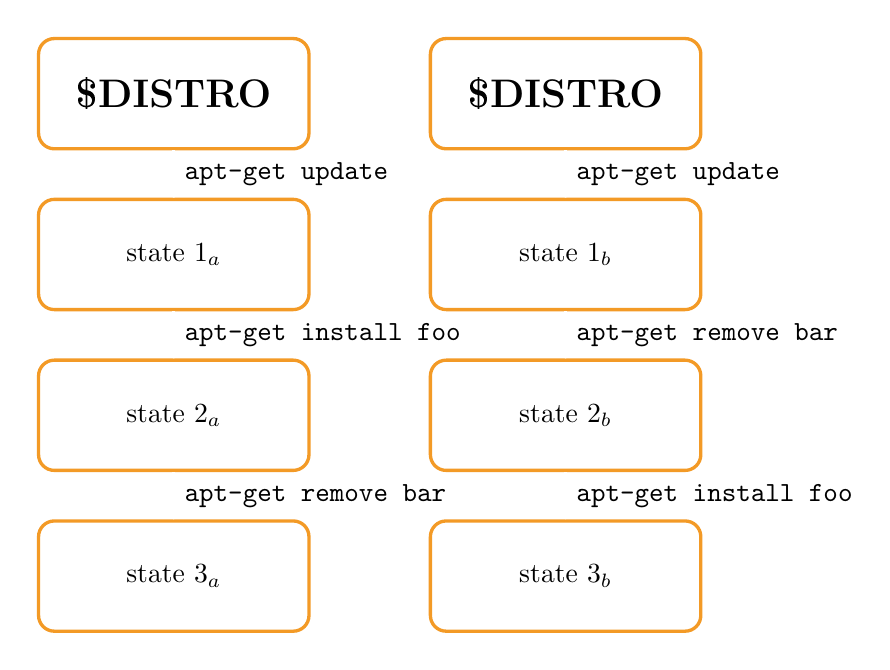
\begin{tikzpicture}[stylish/.style = {
                        draw=guixorange1, very thick,
                        fill=white, text=black, text width=3.2cm,
                        rounded corners=2mm, minimum height=1.4cm,
                        text centered
                      }]
    \matrix[row sep=6mm, column sep=1.5cm] {
      \node(inita)[stylish]{\textbf{\Large{\$DISTRO}}};
      & \node(initb)[stylish]{\textbf{\Large{\$DISTRO}}};
      \\

      \node<2->(state1a)[stylish]{state $1_a$};
      & \node<2->(state1b)[stylish]{state $1_b$};
      \\

      \node<3->(state2a)[stylish]{state $2_a$};
      & \node<3->(state2b)[stylish]{state $2_b$};
      \\

      \node<4->(state3a)[stylish]{state $3_a$};
      & \node<4->(state3b)[stylish]{state $3_b$};
      \\
    };

    \path[->, very thick, draw=white]<2->
      (inita) edge node[right]{\texttt{apt-get update}} (state1a);
    \path[->, very thick, draw=white]<3->
      (state1a) edge node[right]{\texttt{apt-get install foo}} (state2a);
    \path[->, very thick, draw=white]<4->
      (state2a) edge node[right]{\texttt{apt-get remove bar}} (state3a);
    
    \path[->, very thick, draw=white]<2->
      (initb) edge node[right]{\texttt{apt-get update}} (state1b);
    \path[->, very thick, draw=white]<3->
      (state1b) edge node[right]{\texttt{apt-get remove bar}} (state2b);
    \path[->, very thick, draw=white]<4->
      (state2b) edge node[right]{\texttt{apt-get install foo}} (state3b);

  \end{tikzpicture}
  \end{overlayarea}

  \begin{tikzpicture}[overlay]
    \node<5>[rounded corners=4, text centered,
          fill=guixorange1, text width=3cm,
          inner sep=5mm, opacity=.75, text opacity=1,
          drop shadow={opacity=0.5}] at (5, 4) {
            \textbf{\Huge{= ?}}
          };
  \end{tikzpicture}
\end{frame}

\setbeamercolor{normal text}{bg=guixdarkgrey,fg=guixred3}
\begin{frame}[fragile]
  \vspace{2cm}
  \Large{
    \textbf{Functional} package management paradigm:

    \begin{enumerate}
    \item build process = \highlight{pure function}
    \item built software = \highlight{persistent graph}
    \end{enumerate}
  }

  \vfill{}
  \small{
    \textit{Imposing a Memory Management Discipline on
      Software Deployment}, Dolstra et al., 2004 (Nix package manager)
  }
\end{frame}
\setbeamercolor{normal text}{fg=white,bg=black}

\setbeamercolor{normal text}{bg=guixblue2}
\begin{frame}
  \Huge{\textbf{Problem \#2:\\ ``the DSL hell.''}}
\end{frame}
\setbeamercolor{normal text}{fg=white,bg=black}

\begin{frame}[fragile]
  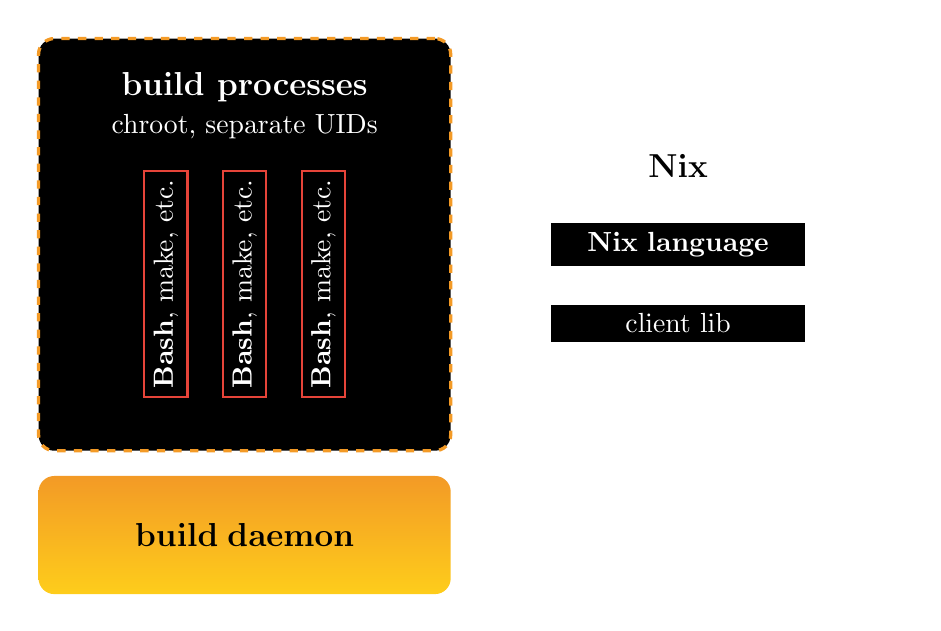
\begin{tikzpicture}[tools/.style = {
                        text width=35mm, minimum height=4cm,
                        text centered,
                        rounded corners=2mm,
                        fill=white, text=black
                      },
                      tool/.style = {
                        fill=black, text=white, text width=3cm,
                        text centered
                      },
                      daemon/.style = {
                        rectangle, text width=50mm, text centered,
                        rounded corners=2mm, minimum height=15mm,
                        top color=guixorange1,
                        bottom color=guixyellow,
                        text=black
                      },
                      builders/.style = {
                        draw=guixorange1, very thick, dashed,
                        fill=black, text=white, text width=5cm,
                        rounded corners=2mm,
                      },
                      builder/.style = {
                        draw=guixred2, thick, rectangle,
                        fill=black, text=white,
                        rotate=90
                      }]
    \matrix[row sep=3mm, column sep=1cm] {
      \node(builders)[builders, text height=5cm]{}
          node[fill=black, text=white] at (0, 2) {\large{\textbf{build processes}}}
          node[fill=black, text=white] at (0, 1.5) {chroot, separate UIDs}
          node[builder, onslide=<1-2>{black}] at (-1,-0.5) {\textbf{Bash}, make, etc.}
          node[builder, onslide=<1-2>{black}] at ( 0,-0.5) {\textbf{Bash}, make, etc.}
          node[builder, onslide=<1-2>{black}] at ( 1,-0.5) {\textbf{Bash}, make, etc.}; &
      \node[tools]{}
          node[fill=white, text=black] at (0, 1) {\large{\textbf{Nix}}}
          node[tool] at (0, 0) {\textbf{Nix language}}
          node(client)[tool] at (0, -1) {client lib};
      \\

      \node(daemon)[daemon]{\large{\textbf{build daemon}}}; &
      &
      \\
    };
  \end{tikzpicture}

  \begin{tikzpicture}[overlay]
    \path[very thick, draw=guixorange1]<2->
      (client.south) edge [out=-90, in=0, ->] node[below, sloped]{RPCs} (daemon.east);
    \path[->, very thick, draw=guixorange1]<3->
      (daemon) edge (builders);
  \end{tikzpicture}
\end{frame}

\begin{frame}[fragile]
  \frametitle{Nix language}

  \vspace{1cm}
  \small{
    \begin{semiverbatim}
\{ \tikz[baseline]{\node[anchor=base](formalparams){fetchurl, stdenv};} \}\tikz[baseline]{\node[anchor=base](colon){:};}

\tikz[baseline]{\node[anchor=base](stdenv){stdenv};}.\tikz[baseline]{\node[anchor=base](funcall){\alert<1>{mkDerivation}};} \{
  name = "hello-2.3";
  src = fetchurl \{
    url = mirror://gnu/hello/hello-2.3.tar.bz2;
    sha256 = "0c7vijq8y68...";
  \};
 \uncover<2->{\tikz[baseline]{\node[anchor=base](bash){preCheck = "echo 'Test suite coming up!'";};}}
  meta = \{
    description = "Produces a friendly greeting";
    homepage = http://www.gnu.org/software/hello/;
    license = "GPLv3+";
  \};
\}
    \end{semiverbatim}
    }

  \begin{textblock}{5}(10, 3)
    \tikz{\node<1>(labelcolon)[fill=white, text=black]{function definition};}
  \end{textblock}

  \begin{textblock}{5}(11, 6)
    \tikz{\node<1>(labelfuncall)[fill=white, text=black]{function call};}
  \end{textblock}

  \begin{textblock}{5}(11, 9)
    \tikz{\node<2>(labelbash)[fill=white, text=black]{Bash snippet};}
  \end{textblock}

  \begin{tikzpicture}[overlay]
    \path[->]<1>(labelcolon) edge (colon);
    \path[->]<1>(labelfuncall) edge (funcall);
    \path[->]<2>(labelbash) edge (bash);
  \end{tikzpicture}
\end{frame}

\screenshot{images/nix-shell-escapes}

\setbeamercolor{normal text}{bg=guixblue2}
\begin{frame}
  \Huge{\textbf{Scheme all the way down.}}
\end{frame}
\setbeamercolor{normal text}{fg=white,bg=black}

\begin{frame}[plain]
  \begin{quotation}
    \noindent
    \LARGE{``Escaping DSL hell by having parentheses all the way down''}
  \end{quotation}
  \vspace{1cm}
  \hfill{-- talk by Tom Hall}\\
  \hfill{\small{\url{https://skillsmatter.com/skillscasts/5488-escaping-dsl-hell-by-having-parenthesis-all-the-way-down}}}
\end{frame}

\begin{frame}[fragile]
  \begin{semiverbatim}
    \small{
(define hello
  (\alert{package}
    (name "hello")
    (version "2.8")
    (source (\alert{origin}
              (method url-fetch)
              (uri (string-append
                    "http://ftp.gnu.org/\textrm{...}/hello-" version
                    ".tar.gz"))
              (sha256 (base32 "0wqd\textrm{...}dz6"))))
    (\alert{build-system} gnu-build-system)
    (synopsis "An example GNU package")
    (description "Produce a friendly greeting.")
    (home-page "https://gnu.org/software/hello/")
    (license gpl3+)))

;; \textsl{Yields: /gnu/store/\textrm{...}-hello-2.8}
}
  \end{semiverbatim}
\end{frame}

\begin{frame}[plain]
  \Large{$\Rightarrow$ plan working
    \textbf{as expected}}
  \\[1cm]
  \uncover<2->{\Huge{\textbf{embed DSLs!}}}
\end{frame}

\begin{frame}
  \Large{
  \begin{itemize}
  \item Emacs and Web user interfaces
  \item \texttt{guix refresh} package auto-updater
  \item \texttt{guix lint} package checker
  \item \texttt{guix graph} dependency graph viewer
  \item \texttt{guix size} package size profiler
  \item ...
  \end{itemize}
  }
\end{frame}

\begin{frame}[fragile]{}
  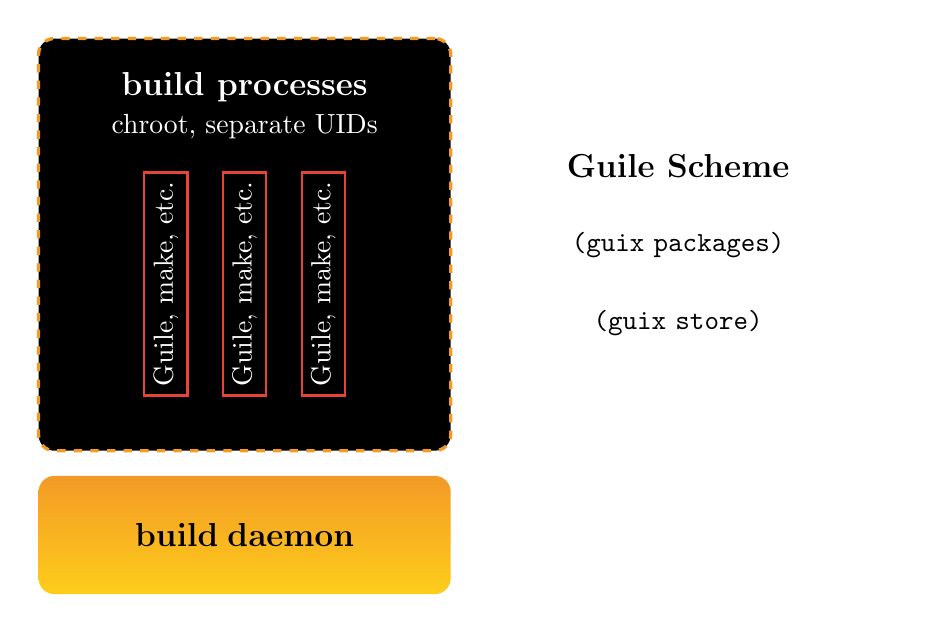
\begin{tikzpicture}[tools/.style = {
                        text width=35mm, minimum height=4cm,
                        text centered,
                        rounded corners=2mm,
                        fill=white, text=black
                      },
                      tool/.style = {
                        fill=white, text=black, text width=3cm,
                        text centered
                      },
                      daemon/.style = {
                        rectangle, text width=50mm, text centered,
                        rounded corners=2mm, minimum height=15mm,
                        top color=guixorange1,
                        bottom color=guixyellow,
                        text=black
                      },
                      builders/.style = {
                        draw=guixorange1, very thick, dashed,
                        fill=black, text=white, text width=5cm,
                        rounded corners=2mm,
                      },
                      builder/.style = {
                        draw=guixred2, thick, rectangle,
                        fill=black, text=white,
                        rotate=90
                      }]
    \matrix[row sep=3mm, column sep=1cm] {
      \node(builders)[builders, text height=5cm]{}
          node[fill=black, text=white] at (0, 2) {\large{\textbf{build processes}}}
          node[fill=black, text=white] at (0, 1.5) {chroot, separate UIDs}
          node[builder] at (-1,-0.5) {\alert{Guile}, make, etc.}
          node[builder] at ( 0,-0.5) {\alert{Guile}, make, etc.}
          node[builder] at ( 1,-0.5) {\alert{Guile}, make, etc.}; &
      \node[tools]{}
          node[fill=white, text=black] at (0, 1) {\large{\textbf{Guile Scheme}}}
          node[tool] at (0, 0) {\texttt{(guix packages)}}
          node(client)[tool] at (0, -1) {\texttt{(guix store)}};
      \\

      \node(daemon)[daemon]{\large{\textbf{build daemon}}}; &
      &
      \\
    };
  \end{tikzpicture}

  \begin{tikzpicture}[overlay]
    \path[very thick, draw=guixorange1]
      (client.south) edge [out=-90, in=0, ->] node[below, sloped]{RPCs} (daemon.east);
    \path[->, very thick, draw=guixorange1]
      (daemon) edge (builders);
  \end{tikzpicture}
\end{frame}

\setbeamercolor{normal text}{bg=guixblue2}
\begin{frame}
  \Huge{\textbf{Unification beyond the ``distro''.}}
\end{frame}
\setbeamercolor{normal text}{fg=white,bg=black}

\begin{frame}{Typical ``Core'' GNU/Linux Stack}
  \Large{
  \begin{itemize}
  \item{ independently-developed daemons/systems code
    \begin{itemize}
    \item<2-> \Large\highlight{inconsist, hard to navigate}
    \end{itemize}}
  \item{little or no code sharing
    \begin{itemize}
    \item<2-> \Large\highlight{redundant, bug-prone}
    \end{itemize}}
  \item{a variety of languages, config syntaxes, etc.
    \begin{itemize}
    \item<2-> \Large\highlight{hard to learn \& master}
    \end{itemize}}
  \item ...
  \end{itemize}
  }
\end{frame}

\begin{frame}[fragile]{Example \#1: the Initial RAM Disk}
  \pause
  \begin{semiverbatim}
(expression->initrd
 (\alert{with-imported-modules} (source-module-closure
                         '((gnu build linux-boot)
                           (guix build utils)))
   \alert{\tikz[baseline]{\node[anchor=base](tilde){#~};}}(begin
       (\alert{use-modules} (gnu build linux-boot)
                    (guix build utils))

       (boot-system #:mounts '\alert{#$}file-systems
                    #:linux-modules '\alert{#$}linux-modules
                    #:linux-module-directory '\alert{#$}kodir)))
  \end{semiverbatim}

  \begin{textblock}{4}(7, 3)
    \tikz{\node<3->(labeltilde)[fill=white, text=black]{\large{\textbf{code staging}}};}
  \end{textblock}

  \begin{tikzpicture}[overlay]
    \path[->, thick]<3-> (labeltilde) edge (tilde);
  \end{tikzpicture}
\end{frame}

\begin{frame}
  \begin{overlayarea}{\textwidth}{8cm}
  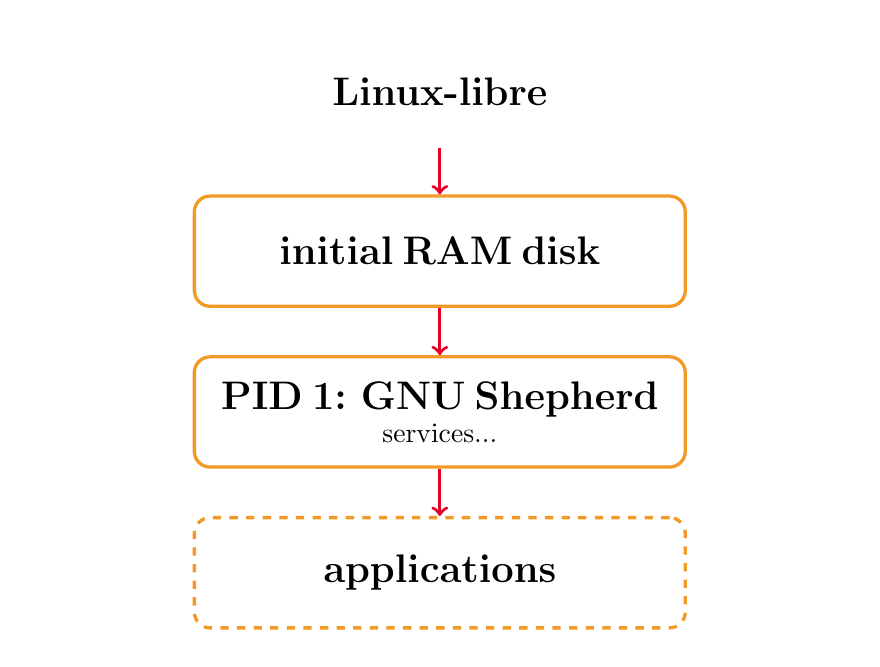
\begin{tikzpicture}[kernel/.style = {
                        text width=10cm, minimum height=1.4cm,
                        text centered,
                        rounded corners=2mm,
                        fill=white, text=black
                      },
                      userland/.style = {
                        draw=guixorange1, very thick,
                        fill=white, text=black, text width=6cm,
                        rounded corners=2mm, minimum height=1.4cm,
                        text centered
                      }]
    \matrix[row sep=6mm, column sep=1cm] {
      \node(kernel)[kernel]{\textbf{\Large{Linux-libre}}};
      \\

      \node<2->(initrd)[userland]{\textbf{\Large{initial RAM disk}}};
      \\

      \node<4->(shepherd)[userland]{\textbf{\Large{PID 1: GNU Shepherd}}
        \\ services...};
      \\

      \node<6->(user)[userland, dashed]{\textbf{\Large{applications}}};
      \\
    };

    \path[->, very thick, draw=guixred1]<2->
      (kernel) edge (initrd);
    \path[->, very thick, draw=guixred1]<4->
      (initrd) edge (shepherd);
    \path[->, very thick, draw=guixred1]<6->
      (shepherd) edge (user);
    
  \end{tikzpicture}
  \end{overlayarea}

  \begin{tikzpicture}[overlay,
                      guile/.style = {
                         fill=guixyellow, text=black, rotate=30,
                         rounded corners=4mm, text width=3cm,
                         opacity=.75, text opacity=1, text centered,
                         minimum height=1.3cm
                      }]
    \node<3->(labelinitrd) [guile] at (initrd.east) {%
      \Large{Guile}
    };
    \node<5->(labelinitrd) [guile] at (shepherd.east) {%
      \Large{Guile}
    };
  \end{tikzpicture}
\end{frame}

\begin{frame}[fragile]{Example \#2: System Services}
  \begin{semiverbatim}
(\alert{shepherd-service}
  (provision '(mysql))
  (documentation "Run the MySQL server.")
  (start (let ((my.cnf (mysql-configuration-file config)))
           \alert{#~}(make-forkexec-constructor
              (list (string-append \alert{#$}mysql "/bin/mysqld")
                    (string-append "--defaults-file="
                                   \alert{#$}my.cnf))
              #:user "mysql" #:group "mysql")))
  (stop \alert{#~}(make-kill-destructor)))
  \end{semiverbatim}
\end{frame}

\setbeamercolor{normal text}{bg=guixblue2}
\begin{frame}
  \Huge{\textbf{Wrap-up.}}
\end{frame}
\setbeamercolor{normal text}{fg=white,bg=black}

\begin{frame}{Summary}
  \Large{
  \begin{itemize}
  \item \highlight{embedding} the distro tools in Scheme is fruitful!
  \item \highlight{hackability} through uniformity
  \item \highlight{code staging} techniques to glue it all
  \end{itemize}
  }
\end{frame}

\begin{frame}{Join us now, share the parens!}
  \vspace{0.7cm}
  \Large{
    \begin{itemize}
    \item \textbf{install the distribution}
    \item \textbf{use it}, report bugs, add packages
    \item share your \textbf{ideas}!
    \end{itemize}
  }
\end{frame}

%%%%%%%%%%%%%%%%%%%%%%%%%%%%%%%%%%%%%%%%%%%%%%%%%%%%%%%%%%%%%%%%%%%%%%%%%%%%%%
\begin{frame}[plain]

\vfill{
  \vspace{2.5cm}
  \center{\includegraphics[width=0.3\textwidth]{images/GuixSD}}\\[1.0cm]
  \texttt{ludo@gnu.org}\hfill{\alert{\url{https://gnu.org/software/guix/}}}
}

\end{frame}

\begin{frame}{}

  \begin{textblock}{12}(2, 8)
    \tiny{
      Copyright \copyright{} 2010, 2012--2016 Ludovic Courtès \texttt{ludo@gnu.org}.\\[3.0mm]
      GNU GuixSD logo, CC-BY-SA 4.0, \url{https://gnu.org/s/guix/graphics}

      Copyright of other images included in this document is held by
      their respective owners.
      \\[3.0mm]
      This work is licensed under the \alert{Creative Commons
        Attribution-Share Alike 3.0} License.  To view a copy of this
      license, visit
      \url{http://creativecommons.org/licenses/by-sa/3.0/} or send a
      letter to Creative Commons, 171 Second Street, Suite 300, San
      Francisco, California, 94105, USA.
      \\[2.0mm]
      At your option, you may instead copy, distribute and/or modify
      this document under the terms of the \alert{GNU Free Documentation
        License, Version 1.3 or any later version} published by the Free
      Software Foundation; with no Invariant Sections, no Front-Cover
      Texts, and no Back-Cover Texts.  A copy of the license is
      available at \url{http://www.gnu.org/licenses/gfdl.html}.
      \\[2.0mm]
      % Give a link to the 'Transparent Copy', as per Section 3 of the GFDL.
      The source of this document is available from
      \url{http://git.sv.gnu.org/cgit/guix/maintenance.git}.
    }
  \end{textblock}
\end{frame}

\end{document}

% Local Variables:
% coding: utf-8
% comment-start: "%"
% comment-end: ""
% ispell-local-dictionary: "american"
% compile-command: "rubber --pdf talk.tex"
% End:
